\documentclass[10pt,letterpaper]{article} 
\usepackage{tikz}
\usepackage{tools}
\usepackage{enumitem,caption}
\usepackage{listings}
\lstset{language=Python}
%\lstset{frame=lines}
%\lstset{caption={Insert code directly in your document}}
\lstset{label={lst:code_direct}}
\lstset{basicstyle=\footnotesize}

%\usepackage{graphicx}‎‎
%\usefonttheme{serif}‎
%\usepackage{ptext}‎
%\usepackage{xepersian}
%\settextfont{B Nazanin}
\usepackage{lipsum}
\setlength{\parindent}{0pt}
\newcommand{\pf}{$\blacksquare$}

\newcommand{\Span}{\text{Span}}
\newcommand{\NF}{\text{NF}}
\newcommand{\EDFA}{\text{EDFA}}
\newcommand{\ASE}{\text{ASE}}

\newcommand{\bns}{\textit{broadcast-and-select}  architecture}
\newcommand{\Bns}{\textit{Broadcast-and-select} architecture}

\newcommand{\rns}{\textit{route-and-select} architecture}
\newcommand{\Rns}{\textit{Route-and-select} architecture}

\newcounter{QuestionNumber}
\setcounter{QuestionNumber}{1}

\newcommand{\temp}{{\color{red}{temp}}}

\newcommand{\Q}{
\textbf{Question \theQuestionNumber)}
\stepcounter{QuestionNumber}
}
\newcommand{\EX}{\Bbb E}
\newcommand{\nl}{\newline\newline}
\begin{document}
\large
\begin{center}
In the name of beauty

The 5th problem set solution of Optical Networks course
\hl
\end{center}
\Q

It is a known fact (and actually can be easily proved) that a linear function $ax+by$ increases for any direction of variation of $(x,y)$ that forms an acute to right angle with the gradient vector $(a,b)$, with the steepest ascent happening when the direction of variation of $(x,y)$ is at the direction of gradient vector. Based on this fact, for solving the LPs (or ILPs), we first sketch the feasible region. Then, we plot the gradient vector and move the contour of objective function in the direction of gradient for maximization problems such that the contour becomes almost leaving the feasible region. The last point (points) of touch between the contour of objective function and the feasible region is regarded as optimal point.

%(Linear Programming)

\begin{figure}[h]
\centering
\begin{subfigure}{0.49\textwidth}
\centering
\includegraphics[width=60mm]{lp1}
\caption{Question 1, part a}
\end{subfigure}
\begin{subfigure}{0.49\textwidth}
\centering
\includegraphics[width=60mm]{lp2}
\caption{Question 1, part b}
\end{subfigure}
\begin{subfigure}{0.49\textwidth}
\centering
\includegraphics[width=60mm]{lp3}
\caption{Question 1, part c}
\end{subfigure}
\end{figure}

\Q

\begin{figure}[h]
\centering
\begin{subfigure}{0.49\textwidth}
\centering
\includegraphics[width=60mm]{ilp1}
\caption{Question 2, part a}
\end{subfigure}
\begin{subfigure}{0.49\textwidth}
\centering
\includegraphics[width=60mm]{ilp2}
\caption{Question 2, part b}
\end{subfigure}
\end{figure}

\newpage

\Q

\begin{enumerate}[label=\alph*-]
\item
A negative loop would lead to infinite iteration in the Bellman-Ford's algorithm, where the path cost would drop at each iteration.

\item
{\color{white}{invisible}}
\begin{figure}[h]
\centering
\begin{subfigure}{0.48\textwidth}
\centering
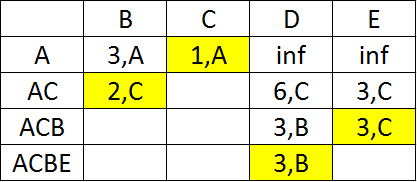
\includegraphics[width=60mm]{dij1.png}
\caption{Dijkstra algorithm for part (a)}
\end{subfigure}
\begin{subfigure}{0.48\textwidth}
\centering
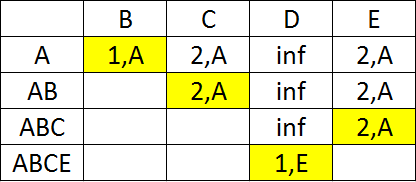
\includegraphics[width=60mm]{dij2.png}
\caption{Dijkstra algorithm for part (b)}
\label{bf}
\end{subfigure}
\end{figure}
\item
{\color{white}{invisible}}
\begin{figure}[h]
\centering
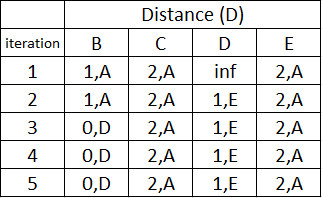
\includegraphics[width=60mm]{bellford.png}
\caption{Bellman-Ford algorithm for part (c)}
\end{figure}
\end{enumerate}
%\begin{figure}[h]
%\centering
%\begin{subfigure}{0.48\textwidth}
%\centering
%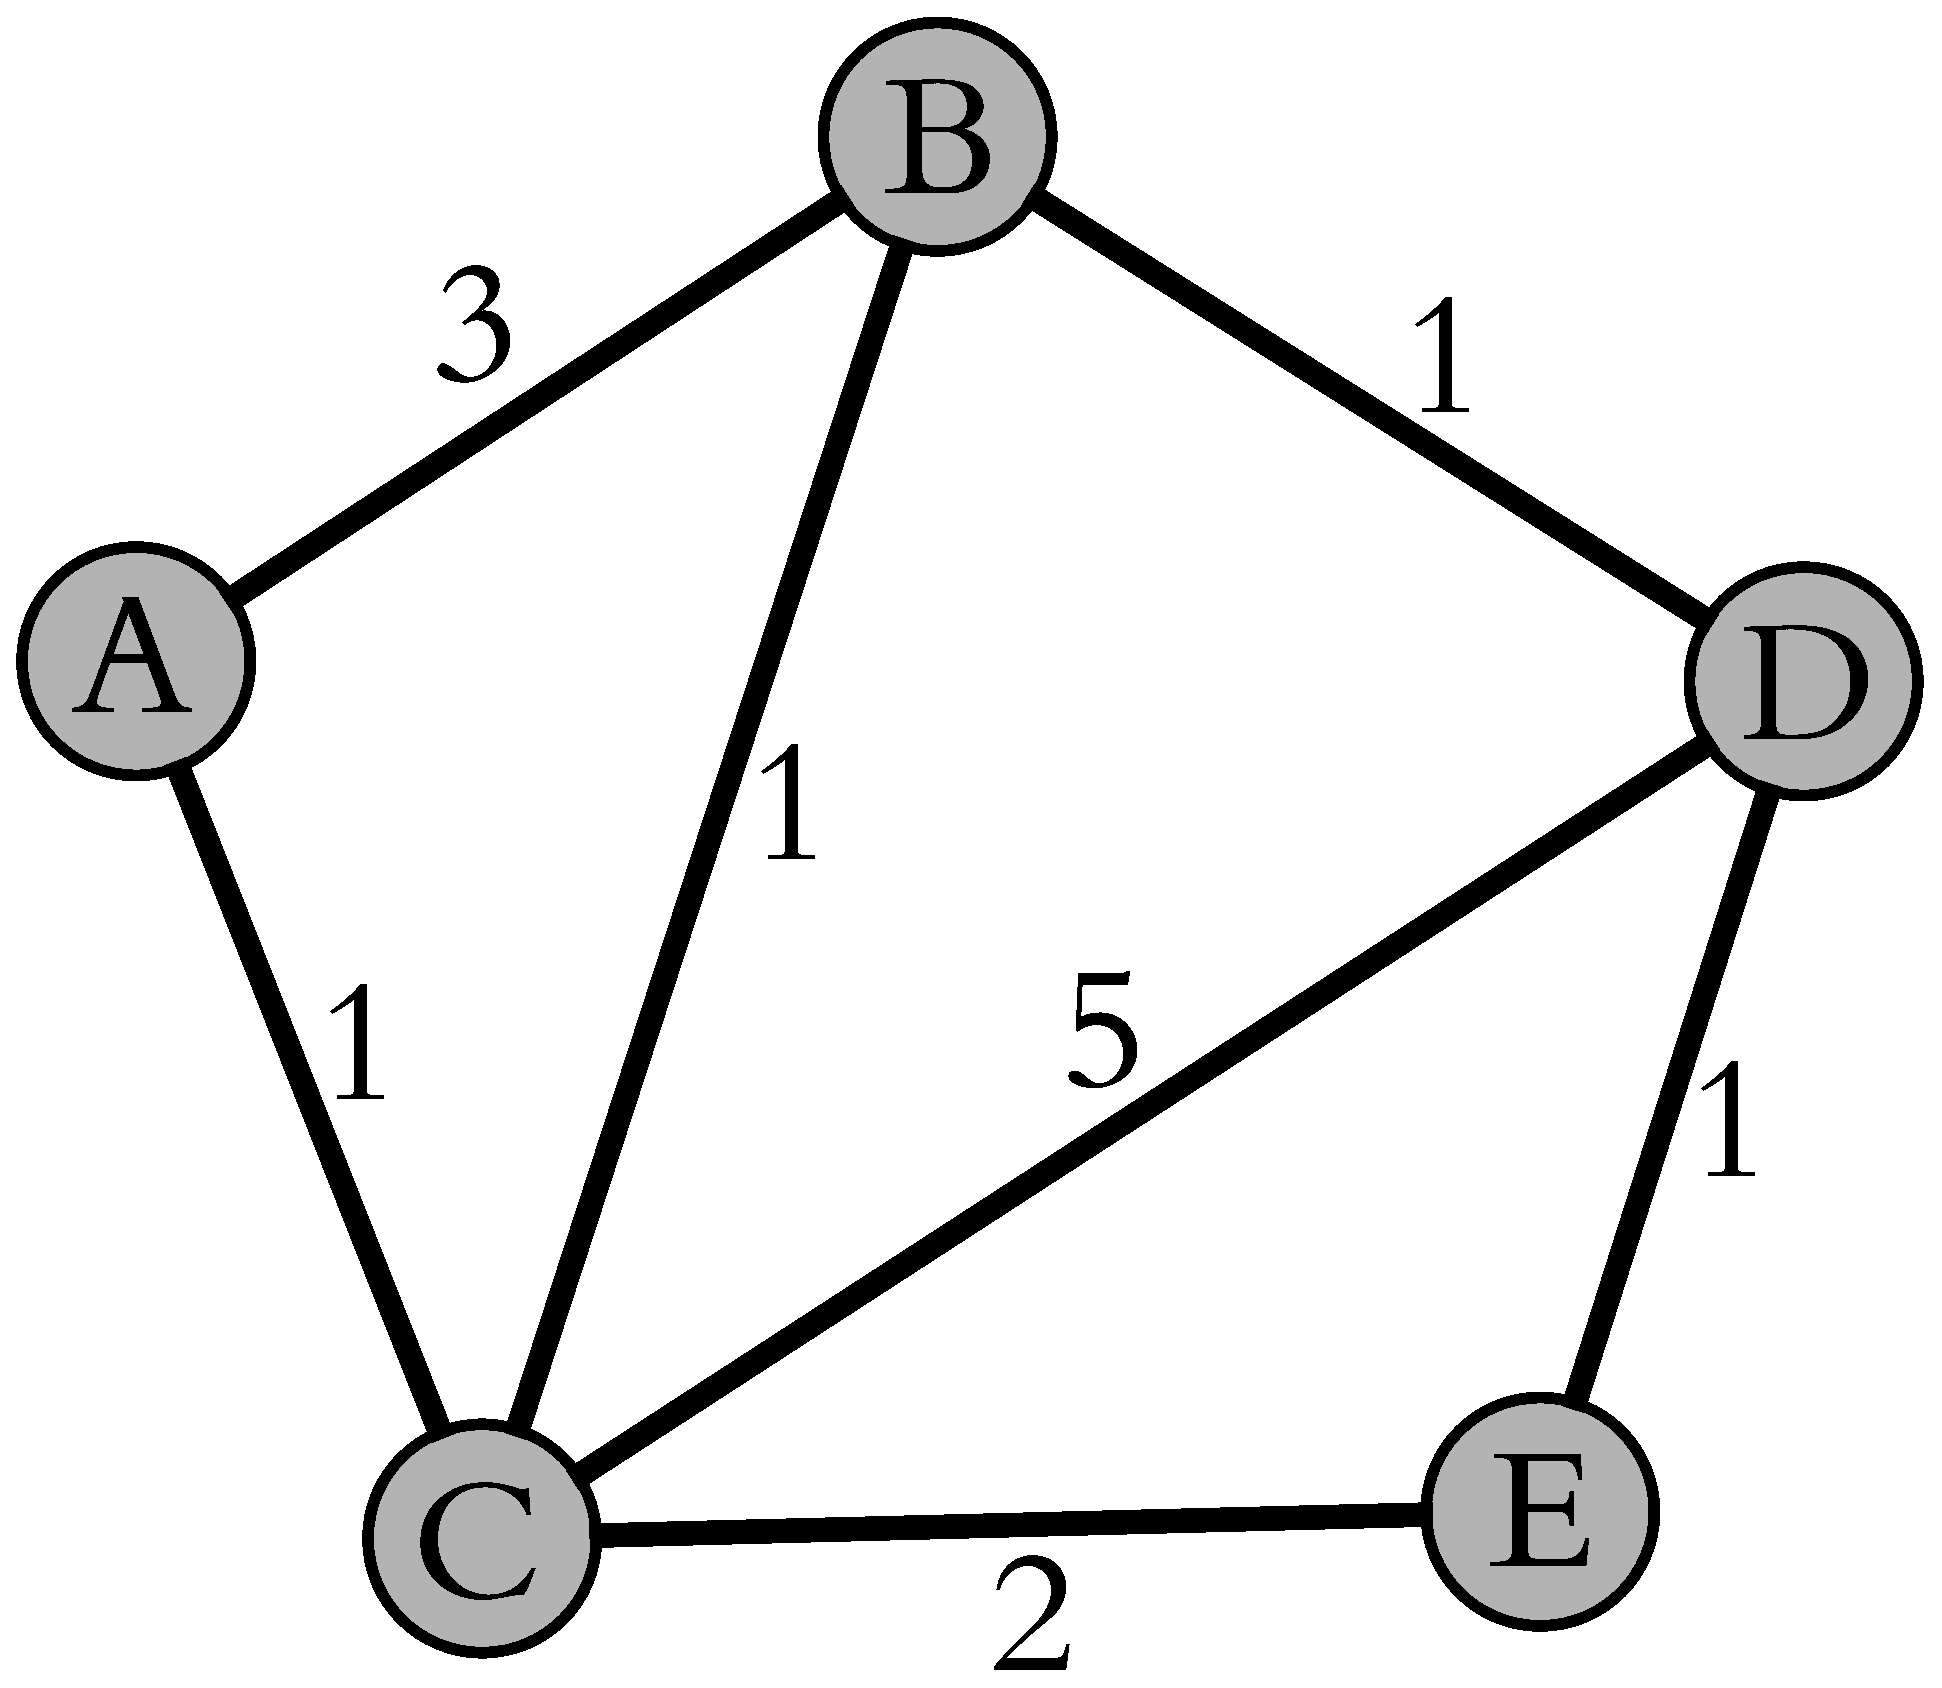
\includegraphics[width=50mm]{Dijkstra.eps}
%\caption{Simple network}
%\end{subfigure}
%\begin{subfigure}{0.48\textwidth}
%\centering
%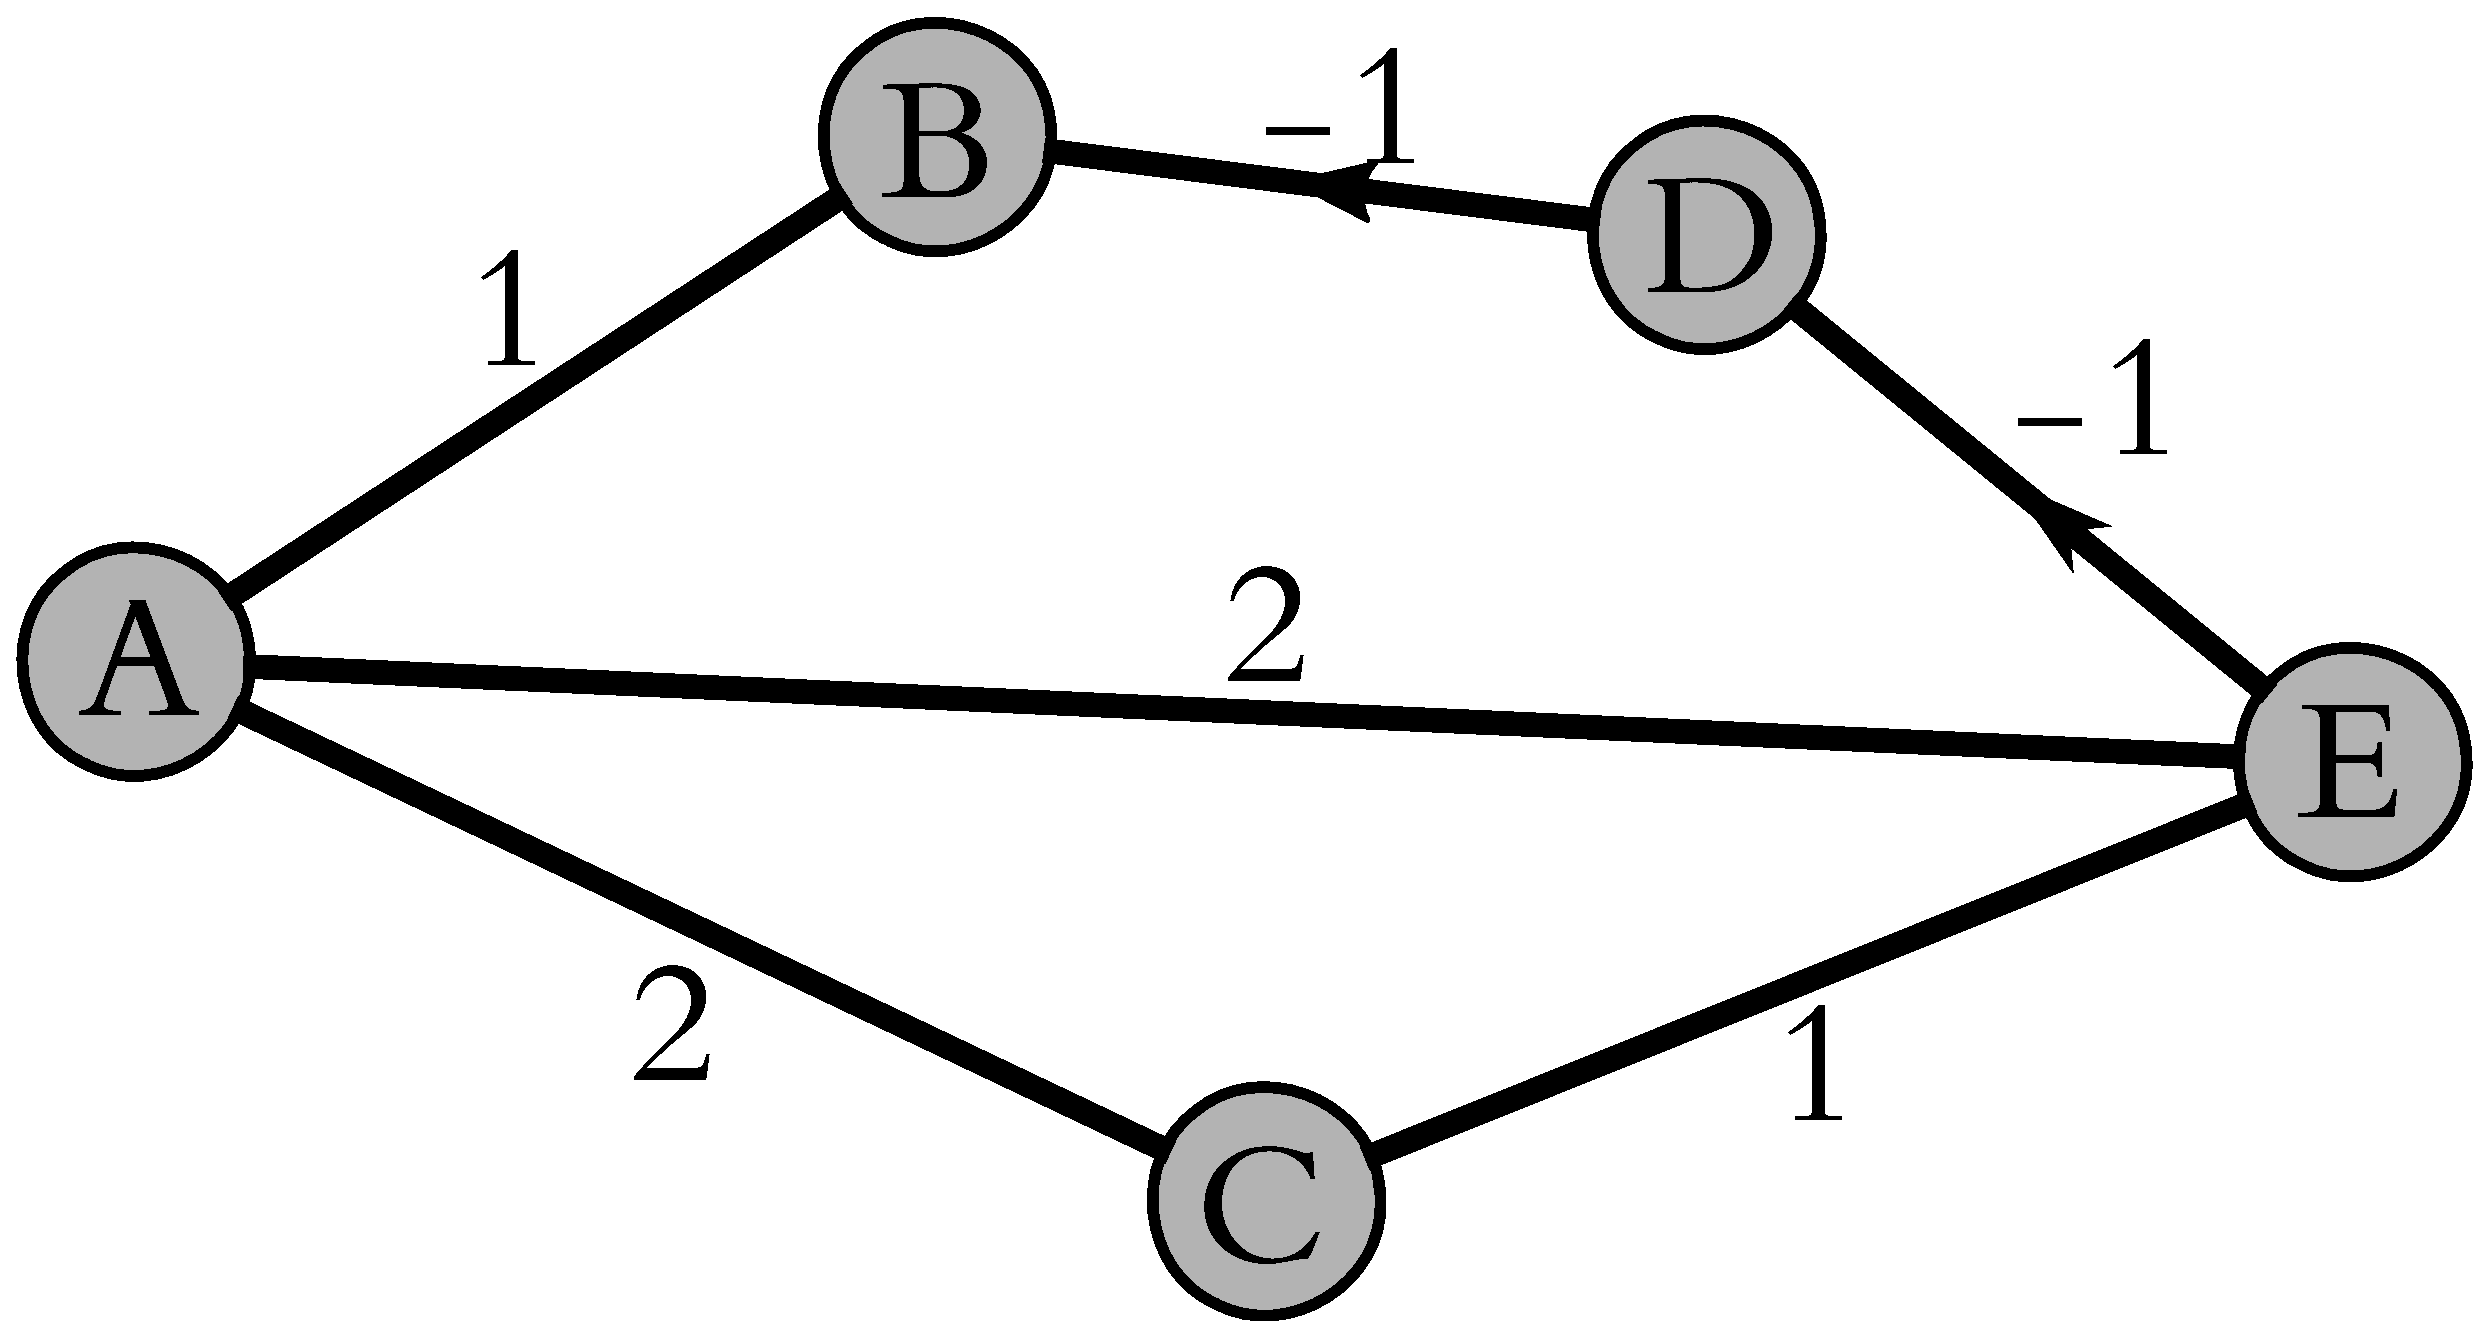
\includegraphics[width=65mm]{Dijkstra_Flawed.eps}
%\caption{Network with positive and negative link costs}
%\label{bf}
%\end{subfigure}
%\caption{}
%\end{figure}

\Q

We wish to solve the max-flow problem in the following network through LP. Our objective is the maximal flow that can traverse the following physical topology.
\begin{figure}[h]
\centering
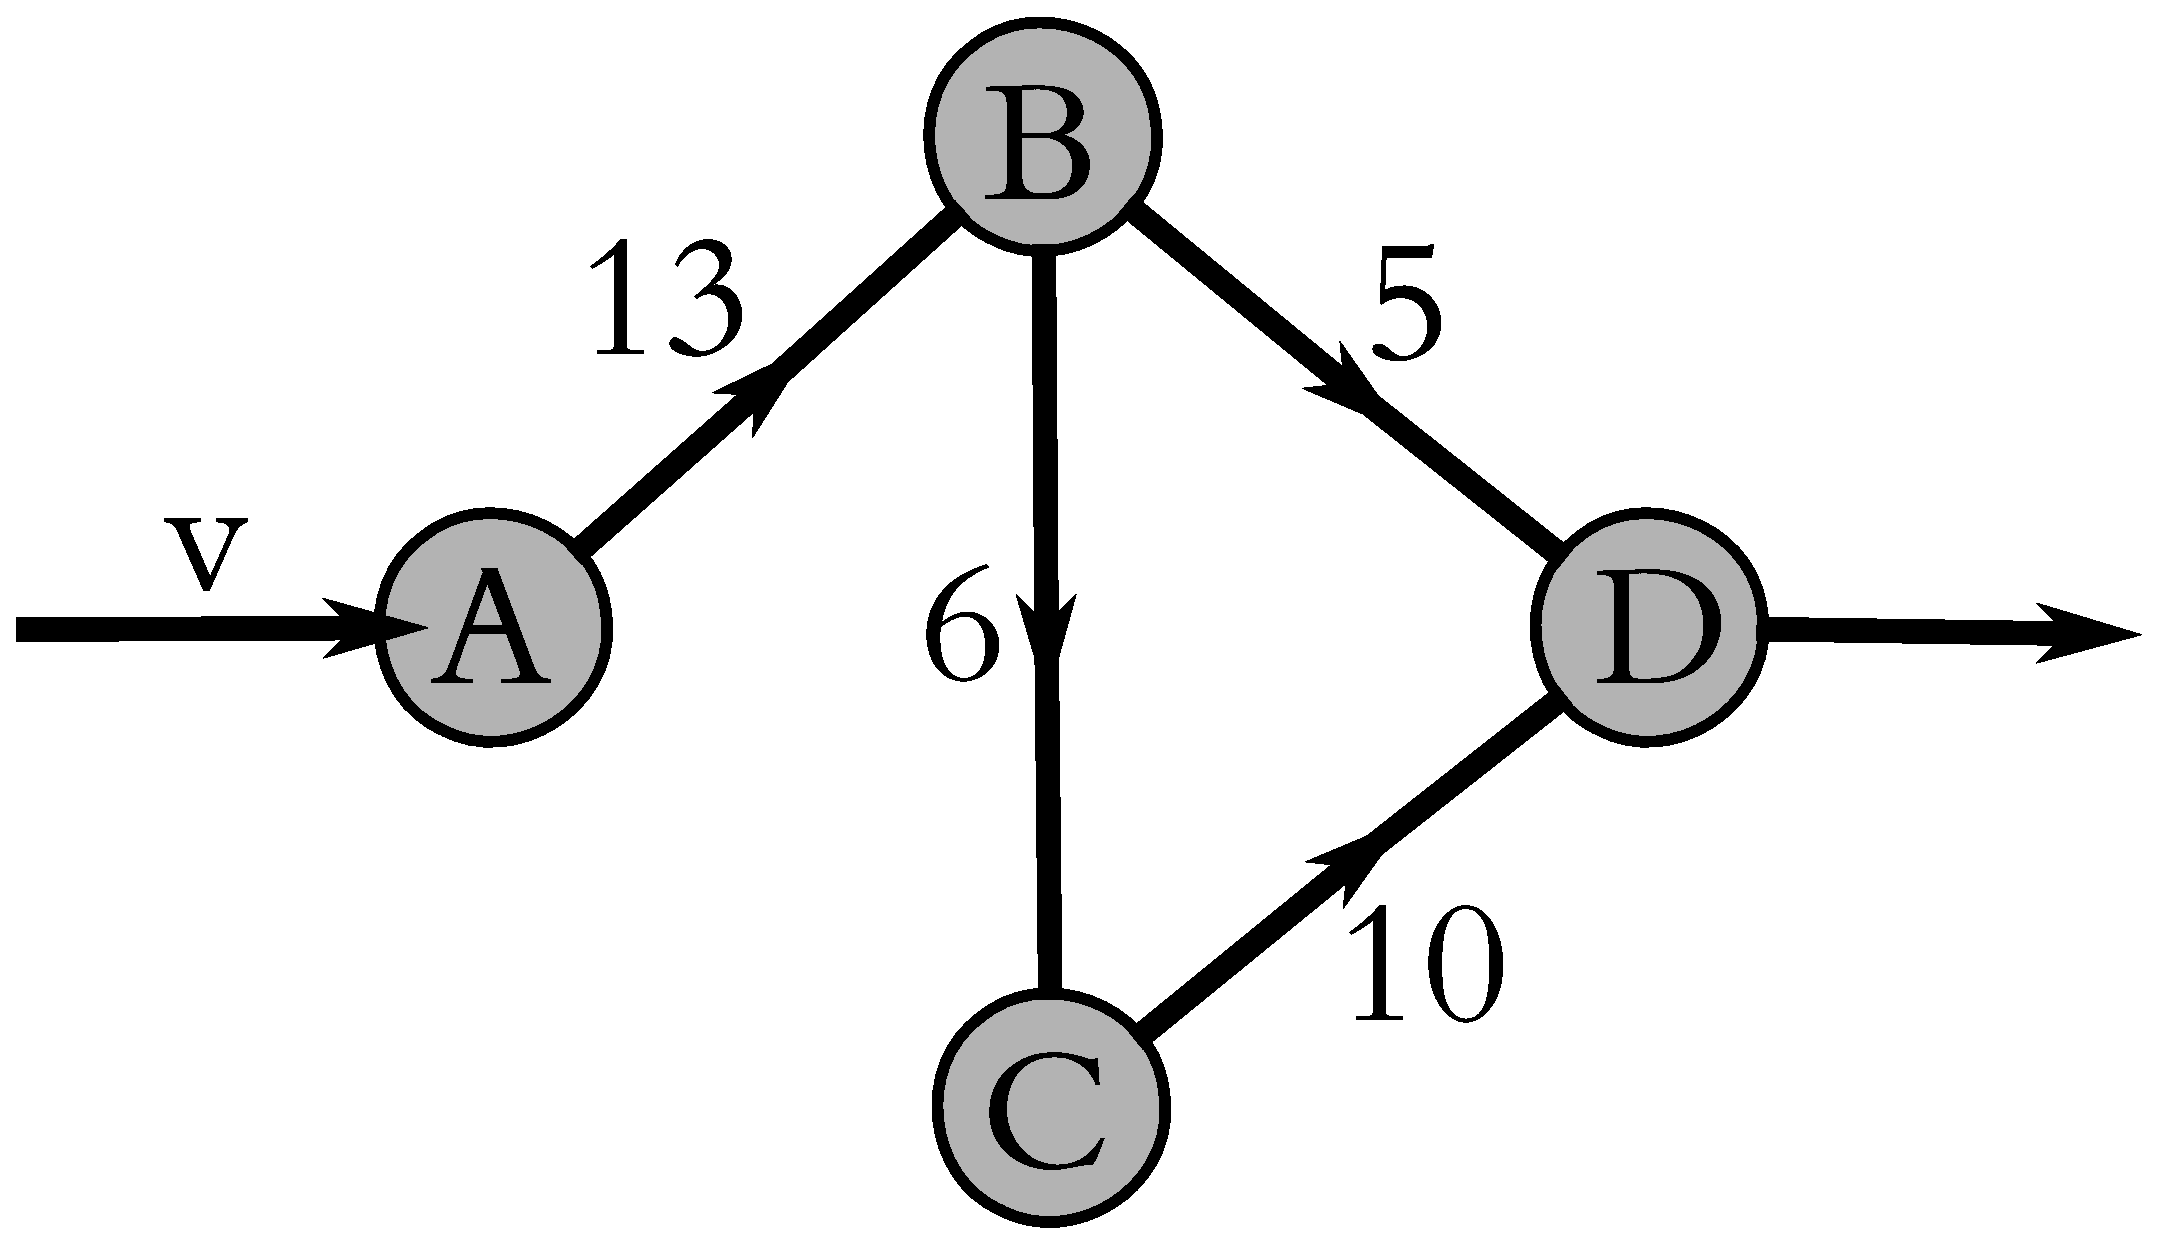
\includegraphics[width=60mm]{max_flow.eps}
\end{figure}
The numbers on each link denote the capacity of the link. Assume the total flow from node i to node j on their direct link is $x_\text{ij}$ and each such flow must not exceed its capacity and is always non-negative, e.g.
$
0\le x_\text{BC} \le 6.
$
The total traffic volume $v$ passes through this network from node A to node D, which should be maximized. Formulate the problem of maximum flow in LP framework and solve it to find the maximum traffic. Section 4.2.1 of ``Linear Programming and Algorithms for Communication Networks'' has discussed this type of LP problems in detail (further simplifications on the problem formulation would leave you with a two-dimensional LP, so you can solve it visually).

An ILP formulation is as follows:
\[
\begin{split}
&\text{maximize} \ \ v
\\&\text{s. t.}
\\&\quad v=x_\text{AB}
\\&\quad x_\text{AB}=x_\text{BC}+x_\text{BD}
\\&\quad x_\text{BC}=x_\text{CD}
\\&\quad 0\le x_\text{AB}\le 13
\\&\quad 0\le x_\text{BC}\le 6
\\&\quad 0\le x_\text{BD}\le 5
\\&\quad 0\le x_\text{CD}\le 10,
\end{split}
\]
which can be simplified to
\[
\begin{split}
&\text{maximize} \ \ x_\text{AB}
\\&\text{s. t.}
\\&\quad x_\text{AB}=x_\text{BC}+x_\text{BD}
\\&\quad 0\le x_\text{AB}\le 13
\\&\quad 0\le x_\text{BC}\le 6
\\&\quad 0\le x_\text{BD}\le 5
\end{split}
\]
with the following answer
\[
\begin{split}
&v=11
\\&x_\text{AB}=11
\\&x_\text{BC}=6
\\&x_\text{BD}=5
\\&x_\text{CD}=6.
\end{split}
\]

\end{document}